\documentclass[letterpaper,twocolumn,amsmath,amssymb,pre]{revtex4-1}
\usepackage{graphicx}% Include figure files
\usepackage{color}

\newcommand{\red}[1]{{\bf \color{red} #1}}
\newcommand{\blue}[1]{{\bf \color{blue} #1}}
\newcommand{\green}[1]{{\bf \color{green} #1}}

\newcommand{\fixme}[1]{\red{[#1]}}
\newcommand{\davidsays}[1]{{\color{red} [\green{David:} \emph{#1}]}}
\newcommand{\renesays}[1]{{\color{red} [\blue{Rene:} \emph{#1}]}}
\newcommand{\jeffsays}[1]{{\color{red} [\blue{Jeff:} \emph{#1}]}}

\newcommand\micron{\ensuremath{\mu\text{m}}}

\begin{document}
\title{Robustness of MinD oscillation in \emph{Escherichia coli} with
  diverse cell shapes}

\author{Jeff B. Schulte}
\affiliation{Department of Physics, Oregon State University}
\author{Rene W. Zeto}
\affiliation{Department of Physics, Oregon State University}
\author{David Roundy}
\affiliation{Department of Physics, Oregon State University}

\begin{abstract}
  The dynamics of the Min-protein system help Escherichia coli
  bacteria regulate the process of cell division by identifying the
  center of the cell.  We model the Min-protein system in bacteria
  that have been forced into unusual flattened shapes, as have
  recently been experimentally observed.  We find that although the
  presence of Min oscillations is robust in a wide variety of cellular
  configurations, the location of the peaks is strongly affected by
  the cellular shape.  In some cases no periodic oscillations are
  observed.  In particular, we find that cellular shapes observed
  experimentally to present irregular oscillations do so in the
  theoretical model, consistently \fixme{or inconsistently?} with
  experiment.  \fixme{In agreement with previous theoretical and
    experimental results, we observe ``rotating'' behavior in certain
    shapes having three corners.}
\end{abstract}

\maketitle

\section{Introduction}
It is vital that during the process of bacterial cell division a cell
avoid minicelling, or splitting into daughter cells with lopsided
volumes.  Instrumental to this process in \emph{Escherichia coli} is a
long FtsZ polymer chain that develops on the cell wall in the center
region of the cell, helping dictate the plane of
division~\cite{adams2009bacterial, lutkenhaus2007assembly}. Previous
experimental studies have shown that the MinC protein, known to
inhibit the FtZ polymer\cite{shen2010examination}, exhibits pole to
pole oscillatory behavior in conjunction with the MinD protein and a
MinE that tends to be more localized in the center of the
cell~\cite{hu1999topological, fu2001mine, shapiro2009and, yu1999ftsz,
  raskin1999rapid}. The MinC protein will then have a higher time
averaged concentration in the cell poles, as opposed to the center
region of the cell, aiding in prohibiting the FtZ from developing in
the wrong region.

Studies have shown that the cell division process is capable of
preventing minicelling for fairly perturbed cell
shapes\cite{touhami2006temperature}. Varma et al. studied one
particular example of a perturbed shape, a three-pronged tube, and
found both experimental and simulation results\cite{varma2008min} that
show oscillation. These oscillations seem to seek out the extreme
poles in the cell shape\cite{corbin2002exploring}
\cite{juarez2010changes}, and effectively prevent minicelling in most
cases. However, Mannik et al. have also shown that there are
limitations to this mechanism\cite{mannik2010bacteria}
\cite{mannik2009bacterial}. One instance of this behavior is
observable when the cell has been forced into a flattened, irregular
shape. Oscillations in this sort of cell shape are far from the
regular sorts of oscillations seen in the computational work done by
Huang et al\cite{huang2003dynamic}, who simulate more regular
shapes. Thus there is an opportunity here to test previously used
simulation models against more extreme experimental cases than have
been seen thus far.  In this paper we apply a deterministic method and
a stochastic method of simulation and compare them against Mannik's
experimental findings.

A significant amount of work has been done to develop protein reaction
and diffusion models that exhibit accurate macroscopic dynamics of the
MinD protein system. Early models involve free proteins that affect
each others' rates of diffusion and membrane attachment, but do not
combine into compound states~\cite{meinhardt2001pattern}.  In 2003
Huang improved upon this work with a simple and very successful
simulation model based on MinD-MinE combination, ATPase hydrolysis,
and MinD membrane attachment that exhibits accurate MinD oscillations
in cylindrical cells~\cite{huang2003dynamic}. In this model
cytoplasmic MinD is more likely to attach to the membrane when MinD is
already clustered there (following observed non-linear attachement of
minD on the cell membrane), and is stationary once attached.  A number
of studies have used an approach similar in that they do not rely on
the ability of MinD to move along the walls and
cluster~\cite{kruse2007experimentalist, meinhardt2001pattern,
  drew2005polymerization, fange2006noise, kerr2006division}, while
studies have been made as well of models which rely on MinD mobility
and attraction on the cell membrane~\cite{kruse2002dynamic,
  howard2005cellular}.  Experimental studies of the Min system's
association with the cell membrane have also been
made~\cite{hsieh2010direct}\cite{mileykovskaya2003effects}.

Variations of the Huang 2003 model that stochasticly account for
variations of molecular interaction \cite{fange2006noise} and
monte-carlo simulations that implement this stochastic version of
Huang's mean field reaction rates confirm the major results obtained
by Huang's model, and more successfully predict experimentally
observed oscillations in round cell
phenotypes~\cite{drew2005polymerization, fange2006noise,
  huang2004min}. Biochemical models of broader scope have also been
used to study the MinD system and show consistent
results.\cite{arjunan2010new}.  However, in general, the results of
the stochastic and monte-carlo simulations have so far yeilded similar
results to those given by Huang's original, deterministic method of
simulation.\fixme{Look at the papers again to verify and this and also
  figure out and cite who says that the stochastic and the
  deterministic methods of simulation have given similar results.
  Saying more about these discussions is needed here, I think.
  Something to the effect that until now there's no compelling reason
  to avoid the deterministic simulations.}

\fixme{Following paragraph is awkward, and I don't think it's needed.}
Studies have shown as well that MinD binds preferentially to regions
enriched with cadiolipin, an anionic phospholipid that collects on
regions of high negative curvature. This mechanism has been
incorporated into other
models.\cite{drew2005polymerization,cytrynbaum2007multistranded,renner2012mind,renner2012mind}
However, this mechanism of combined clustering, phospholipids and MinD
has not been observed in real cells. \cite{halatek2012highly}


\begin{figure}
  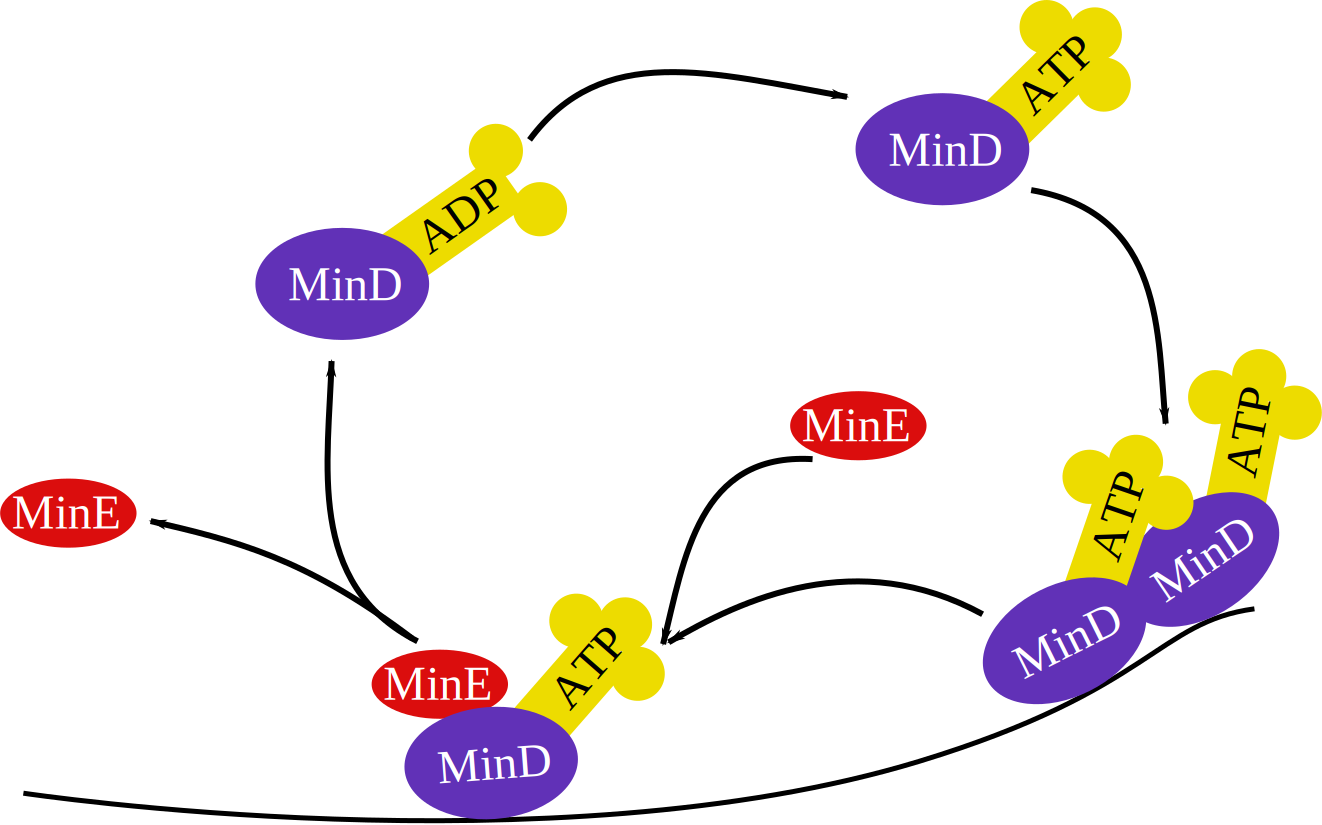
\includegraphics[width=\columnwidth]{reactions}
  \caption{Reactions included in the model of Huang \emph{et
      al.}~\cite{huang2003dynamic}.}\label{fig:reactions}
\end{figure}


\section{Model, Methods, and Cell Shapes}
We implement the reaction-diffusion model of Huang \emph{et
  al.}~\cite{huang2003dynamic}.  Figure~\ref{fig:reactions} shows the
reaction process.  The cytoplasmic MinD:ADP complex undergoes
nucleotide exchange and is changed into the MinD:ATP complex.  This
will naturally diffuse and attach to the cell membrane.  A cytoplasmic
MinE will attach to the wall bound MinD:ATP complex and after a time
will activate ATP hydrolosis.  This breaks up the complex, releasing
MinE, phosphate, and MinD:ADP back into the cytoplasm.  The MinD:ADP
will undergo nucleotide exchange and begin again the cyclic process.
The model is defined by a set of five reaction-diffusion equations:

\begin{multline}
  \frac{\partial \rho_{D:ADP}}{\partial t} = \mathcal{D}_D\nabla^2\rho_{D:ADP}-k_D^{ADP\rightarrow ATP}\rho_{D:ADP}\\
  +\delta(d_w)k_{de}\sigma_{DE},\hspace{3.4cm}
\end{multline}
\begin{multline}
  \frac{\partial \rho_{D:ATP}}{\partial t} = \mathcal{D}_D\nabla^2\rho_{D:ATP}+k_D^{ADP\rightarrow ATP}\rho_{D:ADP}\\
  -\delta(d_w)[k_D+k_{dD}(\sigma_D+\sigma_{DE})]\rho_{D:ATP}
\end{multline}
\begin{multline}
  \frac{\partial \rho_E}{\partial t} = \mathcal{D}_E\nabla^2\rho_E+\delta(d_w)k_{de}\sigma_{DE}
  -\delta(d_w)k_E \sigma_D \rho_E
\end{multline}
\begin{multline}
  \frac{\partial \sigma_D}{\partial t} = -k_E\sigma_D\rho_E
  +[k_D+k_{dD}(\sigma_D+\sigma_{DE})]\rho_{D:ATP}
  \label{eq:d-on-wall}
\end{multline}
\begin{multline}
  \frac{\partial \sigma_{DE}}{\partial t} = -k_{de}\sigma_{DE}+k_E\sigma_D\rho_E\hspace{3cm}
  \label{eq:FifthPDE}
\end{multline}

where $\rho$ is cytoplasmic protein density ($\mu m^{-3}$), $\sigma$
is membrane bound density ($\mu m^{-2}$), $\mathcal{D}_D$ and
$\mathcal{D}_{E}$ th diffusions constants for MinD and MinE,
respectively, $k_D^{\textrm{ADP $\rightarrow$ ATP}}$ the rate of
conversion from MinD:ADP to the MinD:ATP complex, $k_D$ the rate of
MinD:ATP attachement to the membrane when no protein is already
attached there, $k_{dD}$ the increase of this rate when MinD:ATP is
present on the membrane, $k_{de}$ the rate of hydrolisis of the
MinD:MinE:ATP complex, $k_E$ the rate of cytoplasmic MinE binding to
membrane bound MinD:ATP complex, and $d_w$ is the distance from the
point in space to the closest wall (which will always be
perpendicular to this distance).  $\delta(d_w)$ has units of
$\mu m^{-1}$ and will be zero everywhere except at the wall.
Equations \ref{eq:d-on-wall} and \ref{eq:FifthPDE} will only be
relevent at the membrane because the membrane bound density values
will have no meaning in the cytoplasm where there is no membrane.

Our diffusion and reaction rates are shown below.  We are interested
primarily in the effect of cellular size and shape on the protein
oscillations, so we follow Huang\cite{huang2003dynamic} and do not
deviate from the wild type values used in the cited work (see values
below).  Huang's simulations use total MinD and MinE concentrations of
$1,000/\mu m$ and $350/\mu m$, respectively, in a cylindrical cell of
radius $0.5\mu m$, and in our (non-cylindrical) cells we use the same
number of proteins per unit volume.  These concentration values are
1273 $\mu m^{-3}$ and 446 $\mu m^{-3}$, respectively. \fixme{It's been
  a while so might want to check this to make sure it's true.}
\begin{gather*}
  \mathcal{D}_D = \mathcal{D}_{E} = 2.5\micron^2/\text{sec}\\
  k_D^{\textrm{ADP $\rightarrow$ ATP}} = 1/\textrm{sec,  }
  k_D = 0.025 \micron /\textrm{sec}\\
  k_{dD} = 0.0015 \micron^3/ \textrm{sec,  }
  k_{de} = 0.7/\textrm{sec}\\
  k_E = 0.093 \micron^3 /\textrm{sec}.
\end{gather*}
A 3D grid is then constructed in cartesian coordinates, with a grid
spacing of .05\micron.

We have performed both a basic finite analysis, deterministic
simulation that is spatially and temporally discrete, and a stochastic
analysis that is spatially discrete but continuous in time.  Our
stochastic simulation method follows the work of
Kraus~\cite{kraus1996crosstalk} which in turn follows a method
introduced by Gillespie~\cite{gillespie1977exact}.

\begin{figure*}
  %\includegraphics[width=\textwidth]{../data/shape-p/3_00-0_50-0_00-0_00-15_00-exact/plots/image-plot}
  \includegraphics[width=\textwidth]{../data/shape-p/3_00-0_50-0_00-0_00-15_00-exact/plots/single-image-plot}
  \includegraphics[width=\textwidth]{../data/shape-p/3_00-0_50-0_00-0_00-15_00-full_array/plots/single-image-plot}
  \caption{Contour plot images of the concentration of each protein
    species in a natural pill-shaped bacterium at regular intervals in
    time (one second intervals), with darker regions indicating higher
    concentration. The upper plots shows results from the
    deterministic simulation and the lower shows results from the
    stochastic simulation.  The cells pictured are $4\micron$ in
    length, measured from end to end.  The order of frames is such
    that individual MinD proteins begin at the bottom of the plot (in
    the MinD:ATP state in the cytoplasm), and progress upward until
    they reach the MinE:MinD:ATP membrane-bound complex.  At that
    point, they will spontaneously dissociate into cytoplasmic MinE
    (the top row) and the starting state of cytoplasmic MinD:ADP.  The
    densities plotted are integrated along the axis orthogonal to the
    page, and the color scale is chosen separately for each species
    with black as the maximum value over space and time.  The
    stochastic densities are smeared out over space using a guassians
    approximation developed by Zhang et all~\cite{zhang2007gaussian}}.
  \label{image-p}
\end{figure*}

We mean to investigate the geometric limits of the Min system
oscillations as observed by Mannik \emph{et
  al.}~\cite{mannik2012robustness}, so we model the Min system in a
variety of cell shapes and sizes.  Here we present a selection of
these, first naturally occuring pill-shaped cells and then a number of
flattened out shapes which reflect the experiments of Mannik \emph{et
  al.}, in which bacteria are confined within a thin slit of height
$0.25\micron$ ~\cite{mannik2012robustness}. Viewed from the top down
the cells will show the shapes described below and viewed from the
side they show at their edges a semicircular protrusion (one may
imagine the shape of a pancake). We have simulated and analyzed a
number of these flattened shapes in addition to those shown below,
including equilateral and iscosolese triangle shapes, shapes shaped
like greater than signs, '$>$', and four-pronged 'starfish' shapes.
For all of these we have varied the cell size, expanding the two
dimensions that are tangent to the flattened surface from very small,
'steady state' scales (which we discuss below) to scales twice that of
the published Mannik shapes.  Our conclusions are based on all of this
data, but we present here specific, illustrative examples: two
flattened shapes that are designed to replicate those published by
Mannik and two 'stadium' shapes that respectively have the same
quadrupole moments of the two Mannik shapes.

%% Our pill shapes differ from those of Huang \emph{et al.} in that they
%% are cylinders with hemisphere endcaps instead of pure cylindrical
%% shapes.  Our cylinderidrical radius is $0.5\micron$ and the lengths
%% of our cells (measured between the tips of the endcaps) are
%% $5\micron$, $4\micron$, $3\micron$, and $2.5\micron$.

\fixme{Is the following Kubitscheck paragraph needed?}
Kubitschek has shown in multiple experiments that at the time of cell
division cells have a volume that is within a range of roughly
$1\micron^3$ to $2\micron^3$~\cite{kubitschek1990cell,
  kubitschek1968linear}.  We follow Huang's
simulations\cite{huang2003dynamic} and Mannik's experiments and model
cells that are slightly larger than this range.

\section{Naturally Occuring Pill Shaped Cells}

We begin with the naturally occuring pill cell shape.  We peice this
shape together as two hemispherical endcaps attached on either end of
a cylinder.  This shape follows the early simulations of Huang
\emph{et al.} but differs in that we have added the end caps for a
more natural shape, expecting similar results.

This simple cell shape is a good starting point for observing in
detail the dynamic interaction between the different stages of protein
that lead to their qualitatively distinct behavoir. Figure
\ref{image-p} shows the process in a series of frames taken from
simulation animations for both the deterministic and stochastic
simulations.  We have 'smeared out' the stochastic concentrations in a
manner meant to reproduce the images shown by diffraction limited
flourescence microscopy.  We do so using the two dimensional gaussian
approximation developed by Zhang et all~\cite{zhang2007gaussian}.  In
this approximation we use a numerical aperture value of 1.3, which is
the same as used by mannik experimentally, and a wavelength of
$650nm$.  Each frame is 2.5 seconds ahead of the last, and each image
shows the concentration of a given state of protein (of the five
described in the reaction model) summed over the coordinate orthogonal
to the page.  The color scale for each protein state is set according
to the maximum values observed.

Figure~\ref{image-p} begins about 300 seconds into the simulation and
shows a typical period of oscillation that in the pill shape repeates
itself with a high degree of regularity, for both the deterministic
and stochastic simulations.  At $t=0$ the cytoplasmic MinE is
concentrated in the upper portion of the cell and is diffusing
downward, where it will react with and stick to wall-bound MinD that
is concentrated on the membrane in the lower portion of the cell.
This process is in fact already well on its way, as seen by the
significant concentration of wall bound MinD:MinE which is creeping
down to the lower corner, removing the MinD from the membrane as it
goes.  The removed MinD (cytoplasmic MinD:ADP) diffuses freely for a
time before spontenously undergowing nucleotide exchange and shifting
back into the MinD:ATP that is able to attach to the membrane.
Diffusing a small distance away from the bottom of the cell will bring
the protein into the MinE collection, where reactions will prevent it
from collecting for any significant time on the membrane.  Diffusing
further towards the upper end, however, while the MinE has not yet
collected there, will allow MinD:ATP to accumulate with the other
MinD:ATP, which is seen at seconds 10 through 15 in
Figure~\ref{image-p}.  Eventually the MinE creeps all the way down to
the bottom of the cell where it slowly runs out of wall bound MinD to
react with, before diffusing back up and starting again on the upper
portion of the cell. This is seen in seconds 15 through 20 in the
figure.  \fixme{There is another paragraph after this in the latex
  that I commented out because I thought we might be spending too much
  time on the description}

%%  At 15 seconds, the membrane-bound MinD:ATP has
%% been essentially removed from the top end of the cell, and MinD:ATP
%% has begun to bind to the membrane in the the lower half of the cell.
%% At this stage, there is a high concentration of cytoplasmic MinE at
%% the top of the cell, and by 16 seconds we begin to see the formation
%% of a MinE ring just below the center of the cell.  At 18 seconds, the
%% cell has reached its original state (reversed directionally), with
%% MinD:ATP bound to the membrane on the lower third of the cell, a high
%% concentration of cytoplasmic MinE in the upper half of the cell, and a
%% MinE ring pushing downward on the membrane-bound MinD:ATP.

We test cells of radius $.5\micron$ and of lengths $2\micron$,
$3\micron$, $4\micron$, and $5\micron$ measured from the tip of one
end cap to the tip of the other \fixme{I'm running the 2,3,5 pills
  again to make sure that everything in this paragraph is true}. In
each case, we observe in the deterministic simulations a quick
establishement (within a few periods) of extremely regular oscillatory
behavoir that lasts indefinitely.  The stochastic results show
oscillitions that are similarly regular in time, with periods that
nearly match those of the deterministic (they differ roughly by a
factor of .05) \fixme{does this square with the correlation data
  periods?}. The regularity of the pill shape cell periods is
discussed below, in our analysis of time correlation data \fixme{not
  written yet}.  These periods increase with cell length, as shown in
Table~\ref{tab:pill-periods}, in agreement with the results of Huang
\emph{et al.}.

\begin{figure}
  \includegraphics[width=\columnwidth]{../data/shape-p/3_00-0_50-0_00-0_00-15_00-full_array/plots/correlation-rl.pdf}
  \caption{No caption}
  \label{corr-pill}
\end{figure}

While the stochastic results show periods that seem to have a high
degree of regularity as well as similarity to the deterministic
results, they do differ in the precise locations of the maxima.  While
the deterministic simulations show maxima that are every time
concentrated in the center of one of the cell ends, with a symmetric
smear of protein going out laterally to either side, the stochastic
simulations show maxima that, while always located somehwere in the
end region of the cell, occur at different positions within this
region.  This is reflected in Figure~\ref{image-p}, which shows
periods that are the same and qualitative behavoir that is
approximately the same, but also that there is variation in the
details of the stochastic simulation maxima location.

\begin{table}
  \begin{tabular}{|r|c|c|c|l|}
    \hline Length($\mu$) & 2.50 & 3.00 & 4.00 & 5.00\\ \hline
    Period(sec) & sim & 33 & 38 & 48 \\ \cline{2-2} \hline
  \end{tabular}
  \caption{Period of oscillation according to length of cell for
    pill-shaped cells.}\label{tab:pill-periods}
\end{table}

\fixme{Originally the 'Stability Analysis' section came next.  I would
  like to still mention the results of this, since Huang only did the
  analysis on the cylinders, and we've done it on the flattened shapes
  and shown that it works with those too.  But I don't know where to
  fit in the paragraph or so that it would take.  For now I've just
  put the whole section at the end of the paper.}

\begin{figure*}
  \centering
  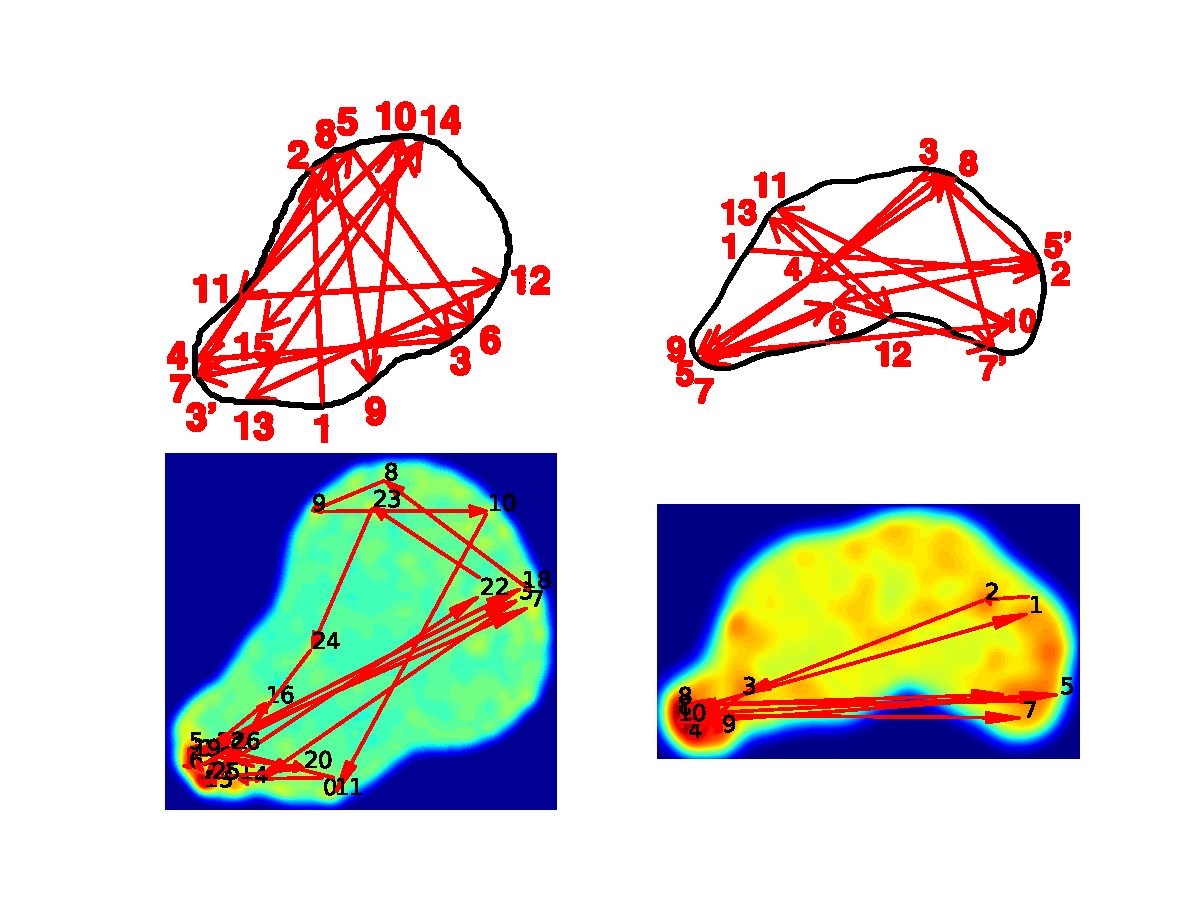
\includegraphics[width=\textwidth]{../paper/plot-ave}
  \caption{Arrows depicting global maxima in space and local
    maxima in
    time overlayed on color plots of time averaged total MinD density.
    A density threshold is chosen and only maxima above this threshold
    are shown. The plots serve to illistrate what is observed in our
    movies.  The simulation time covered in these is 1000 seconds
    \fixme{this is not true yet - need to change the data once its
      finished right now 2 of them are 1000 the others are like 980}.
    The top row shows plots published by Mannik of the MinD maxima
    behavoir and the bottom two rows show our pancake shapes that are
    designed to have the same shape.  The middle row shows results
    from the stochastic simulation and the bottom shows results from
    the deterministic.  We can see that the stochastic method shows
    behavoir that is similar to experiment while the deterministic
    method shows maximization that is too regular and robust.}
  \label{randst-plot-ave}
\end{figure*}

\section{Comparison of Mannik's Experimental and Our Stadium Shapes}

We have made and analyzed movies out of the MinD
concentration that are constructed as those in Figure~\ref{image-p},
integrated along the flattened axis, in which each frame is seperated
in simulation time by a half second. Figure~\ref{randst-plot-ave}
illustrates what is seen in these movies. In his work Mannik presents
arrow plots in which the arrow heads show the location of sequential
MinD maxima within the cell. His plots for his two abnormal cell
shapes are shown in the upper 'experiment' section of
Figure~\ref{randst-plot-ave}.  Following this, we have created plots
that show maxima that are global in space and local in time.  Of these
maxima we only show those which have greater concentration than a
chosen cutoff concentration, and also ignore maxima that appear
temporaly and spatially adjacent to preceding maxima, in order to
stop single spikes from appearing as many adjecent ones.  The overall
effect is to accurately describe what is seen in our movies.

We have found that the deterministic simulations of the protein
reaction sequence discussed above results in robust oscillatory
behavoir of polar selection and oscillation in not only symmetrical
shapes, such as the wildtype pill shape, but also in very
assymetrical, flatttened cells, such as those studied by Mannik.
After the lower size stability limit of
section~\ref{sec:stability-analysis} \fixme{this needs to be covered}
has been surpassed, this qualitative behavoir doesn't seem to have
size dependence until cells reach sizes that have more than twice the
dimensions of the Mannik cells.  At this point the robust
oscillations, while still evident, begin to lose their consistency.
The Mannik reported cells already seem to be rather large (wild type
cells are typically smaller than those observed my Mannik
\cite{kubitschek1990cell,kubitschek1968linear,mannik2012robustness}),
so we left off simulating cells any larger than twice this size.

Looking at Mannik's shape A in Figure~\ref{randst-plot-ave}, we can
see that the deterministic simulation selects out two poles, one at
either end of the cell, and that the MinD does not ever maximize in
any other location.  All of the flattened cells shown in the figure
span a time of 350s (as do Mannik's plots), which corresponds to
\fixme{number of periods} periods for shape A.  The movies show sharp
peaks at these poles, followed by a spreading out of the MinD out into
the cell, with no real bias towards any location, until it aggregates
again at the opposite pole, maximizing there.  The pattern is repeated
again and again with surprising consistency, \fixme{talk about the
  time correlation for the deterministic, once the plots are added.}

The results of these deterministic simulations for shape A differ
significantly with Mannik's experimental results that show much less
regular behavoir, with a large variation in the location of maxima,
shown in the experiment section of Figure~\ref{randst-plot-ave}.

The deterministic results of shape B are slightly different, as can be
seen in the figure.  Here we can see that the proteins maximize on the
rightward cell wall while on the way to their corner maxima locations.
Watching the movies, the proteins seem to travel along the wall, from
corner to corner and back.  This behavoir is still more irregular than
that of the Mannik experiments, which seem to show some right-left
back and forth behavoir in a few areas, as opposed to the straight
pole to pole (traveling along the wall).

These comparisons illustrate our first finding, which is that in
irregular cell shapes, the deterministic method of simulation is indeed
inadequate in representing and predicting experimental behavoir.

On the other hand, our stochastic simulations show both robust pole to
pole oscillations in the symmetric cells and irregular behavoir in the
assymetrical shapes, agreeing well with Mannik's experimental
findings.

Figure~\ref{arrow-pill-stadium} and Figure~\ref{randst-plot-ave} show
color plots of time-averaged MinD overlayed by arrows depicting
sequential maxima that are global in space and local in time.  Our
stochastic method movies (and arrow plots of
Figure~\ref{randst-plot-ave}) show irregular location of maxima that
is similar to what is observed experimentally by Mannik. There is a
general bias towards back and forth behavoir, which can be seen in the
box plots of Figure~\ref{box-mannik}, but the behavoir is irregular
and the location of the maxima vary a significant amount.  On the
other hand, the deterministic simulations show behavoir that is much
too regular when compared with experiment, exhibiting locations of
maxima that do not vary.  The deterministic method is seen to be
inadequate.

Judging that at this point that we have a fair idea of how our two
methods compare with experiment, we investigate the limits of the
break down of regular activity, by simulating large, regular,
'stadium' shapes.  These shapes have the flattened, pancake like form
of the assymetric cells, but from the top down they look as pills
do. In two dimensions they are composed of a rectangle with two half
ellipse connected on either end.  They are also made to have a large
volume that is similar to the Mannik shapes.

We find that both the stochastic and the deterministic solutions show
regular back and forth oscillations in the stadium shaped cells, as
can be seen Figure~\ref{box-stadium}.  This suggests that it is the
irregular, assymetric shape of the Mannik cells, not their size or
their flattened nature, that causes these cells to exhibit
irregularity in MinD oscillations.

%% \begin{figure}
%%   \includegraphics[width=\columnwidth]{../data/shape-stad/0_25-5_50-1_00-0_00-15_00-full_array/plots/box-plot_D}
%%   \includegraphics[width=\columnwidth]{../data/shape-stad/0_25-5_50-1_00-0_00-15_00-exact/plots/box-plot_D}
%%   \caption{A comparison of our box plots that show the similarity
%%     between the stadium shapes simulated stochastically and
%%     deterministically.  Both show regular oscillatory maxima with
%%     similar periods.  This is in contrast to our boxpplot comparison
%%     of one of the Mannik shapes in Figure~\ref{box-mannik}}
%%   \label{box-stadium}
%% \end{figure}


%% \begin{figure}
%%   \includegraphics[width=\columnwidth]{../data/shape-randst/0_25-18_50-18_50-95_00-15_00-full_array/plots/box-plot_D}
%%   \includegraphics[width=\columnwidth]{../data/shape-randst/0_25-18_50-18_50-95_00-15_00-exact/plots/box-plot_D}
%%   \caption{A comparison of our box plots that show a disparity between
%%     the behavoir of the stochastic and deterministic simulations in
%%     our Mannik cells.  The deterministic show a regular, robust
%%     oscillatory behavoir between the two ends of the cell. The
%%     stochastic simulation do show a general back and forth tendency
%%     between two ends of the cell, but it is not robust and tends to
%%     break down.}
%%   \label{box-mannik}
%% \end{figure}
%% \begin{figure}
%%   \includegraphics[width=\columnwidth]{../data/shape-randst/0_25-18_60-28_60-94_00-15_00-full_array/plots/box-plot_D}
%%   \includegraphics[width=\columnwidth]{../data/shape-randst/0_25-18_60-28_60-94_00-15_00-exact/plots/box-plot_D}
%%   \caption{A comparison of our box plots that show a disparity between
%%     the behavoir of the stochastic and deterministic simulations in
%%     our Mannik cells.  The deterministic show a regular, robust
%%     oscillatory behavoir between the two ends of the cell. The
%%     stochastic simulation do show a general back and forth tendency
%%     between two ends of the cell, but it is not robust and tends to
%%     break down.}
%%   \label{box-mannik}
%% \end{figure}


\fixme{specifically design other arrow plot (with many comparisons) to
  illustrate point}


Figure~\ref{arrow-compare-mannik} shows plots of total MinD
concentration maxima that are global in space and local in time.  The
tip of an arrow represents one of these maxima and the adjacent arrow
(whose tail is touching the previous arrow's tip) points to the next
such maxima in time.  Mannik \emph{et al.} have published similar
plots of two of their cells, and we have attempted to replicate the
shape of these cells in our simulation in order to compare.  We find
that when we replicate the size as well as shape of their cells as
near as possible, we do not see the disordered protein behavoir that
they observe.  Instead we see a robust ability of the cell to find two
prefered pole locations and to oscillate maxima back and forth very
steadily between them.  When we increase the size of our cells, we
indeed see multiple positions of maxima develop, but we never observe
the random behavoir that they have observed experimentally.  This is
perhaps due to the exact, continuous method we use when conducting
simulations.  Stochastic methods would perhaps show more random
behavoir at these sizes.  We consider this to be a limitation of the
exact solution method.

\fixme{should I say anything about different/large sizes?}

\begin{figure}
  \includegraphics[width=\columnwidth]{../data/shape-randst/0_25-18_50-18_50-95_00-15_00-full_array/plots/correlation-rl.pdf}
  \includegraphics[width=\columnwidth]{../data/shape-stad/0_25-2_35-1_32-0_00-15_00-full_array/plots/correlation-rl.pdf}
  \caption{Correlation for A shapes}
  \label{corr-A}
\end{figure}


\section{Stability Analysis}
\label{sec:stability-analysis}
We have found that in both methods of simulation there is a lower
length scale that characterizes much of the behavoir.  Regular
oscillatory behavoir between two poles at opposite ends of the longer
cellular direction is found in cells which are long enough in one
dimension for the reaction chain to be unstable but short enough in
the perpendicular dimension to be stable.  The limits are seen when
both dimensions are too short to be unstable, so that initial
assymetry in protein concentration relaxes into a state of no
oscillation.  In these cell sizes, the deterministic simulations show
a motionless steady state and the stochastic simulations show random
fluctuations without any bulk behavoir (see Figure~\ref{box-mannik}).

In order to explain this theoretically, we have performed stability
analysis of the five differential equations in an infinite slab that
show a characteristic half wavelength in perturbative spatial
oscillations at which the system becomes unstable.  This length is
dependent upon slab thickness as shown in
Figure~\ref{fig:stability-analysis}.  When increasing the lengths and
widths of our simulated flattened cells, the cells stop exhibiting two
pole oscillalitory behavior and instead exhibit multiple positions of
maximization when the shortest distance across the cell is
approximately equal to the characteristic half wavelength at the
particular thickness at which we simulate (our simulations of cells
with thickness $0.25\mu m$ corresponds to half wavelengths of $2.13\mu
m$).  Huang~\cite{huang2003dynamic} performs a similar analysis for a
cylindrical shape \fixme{is it cylindrical or 1d?} and finds
characteristic half wavelengths of $2\mu m$.


Decreasing the cell size in succesive steps, we can see the critical
size at which the cell oscillations are quickly damped out.
Figure~\ref{box-mannik} shows box plots of the largest cells simulated
whose oscillations relax into the steady state solution.  Both have a
long axis of roughly 2.2$\mu m$, in agreement with theory.

\section{Conclusion}
No conclusion :(
\begin{figure}
  \includegraphics[width=\columnwidth]{../data/shape-randst/0_25-18_60-28_60-94_00-15_00-full_array/plots/correlation-rl.pdf}
  \includegraphics[width=\columnwidth]{../data/shape-stad/0_25-2_92-1_18-0_00-15_00-full_array/plots/correlation-rl.pdf}
  \caption{Correlation for B shapes}
  \label{corr-B}
\end{figure}

\bibliography{paper}



\end{document}

\section*{Appendix}


\section{Below are NOTES for the Writing}


\end{document}
